%
% The first command in your LaTeX source must be the \documentclass command.
\documentclass[sigconf]{acmart}

%
% defining the \BibTeX command - from Oren Patashnik's original BibTeX documentation.
%\def\BibTeX{{\rm B\kern-.05em{\sc i\kern-.025em b}\kern-.08emT\kern-.1667em\lower.7ex\hbox{E}\kern-.125emX}}
    
% Rights management information. 
% This information is sent to you when you complete the rights form.
% These commands have SAMPLE values in them; it is your responsibility as an author to replace
% the commands and values with those provided to you when you complete the rights form.
%
% These commands are for a PROCEEDINGS abstract or paper.
\copyrightyear{2019}
\acmYear{2019}
\setcopyright{acmlicensed}
\acmConference[COLX 585]{Woodstock '18: ACM Symposium on Neural Gaze Detection}{Trends in Computational Linguistics }{Final Project}
\acmBooktitle{Woodstock '18: ACM Symposium on Neural Gaze Detection, June 03--05, 2018, Woodstock, NY}
\acmPrice{15.00}
\acmDOI{10.1145/1122445.1122456}
\acmISBN{978-1-4503-9999-9/18/06}

%%%%%%%%%%%%%%%%%%%%%%%%%%%%%%%%%%%%%%%%%%%%%%%%%%%%%%%%%%%%%%%%%%%%%%%%%%%%%%%%%%%%%%%%%%%%%%%%%%%
%%                    self added packages                                                        %%
%%%%%%%%%%%%%%%%%%%%%%%%%%%%%%%%%%%%%%%%%%%%%%%%%%%%%%%%%%%%%%%%%%%%%%%%%%%%%%%%%%%%%%%%%%%%%%%%%%%
\usepackage{listings}
\lstset{
	basicstyle=\small\ttfamily,
	columns=flexible,
	breaklines=true
}
\usepackage{multirow}


%
% These commands are for a JOURNAL article.
%\setcopyright{acmcopyright}
%\acmJournal{TOG}
%\acmYear{2018}\acmVolume{37}\acmNumber{4}\acmArticle{111}\acmMonth{8}
%\acmDOI{10.1145/1122445.1122456}

%
% Submission ID. 
% Use this when submitting an article to a sponsored event. You'll receive a unique submission ID from the organizers
% of the event, and this ID should be used as the parameter to this command.
%\acmSubmissionID{123-A56-BU3}

%
% The majority of ACM publications use numbered citations and references. If you are preparing content for an event
% sponsored by ACM SIGGRAPH, you must use the "author year" style of citations and references. Uncommenting
% the next command will enable that style.
%\citestyle{acmauthoryear}

%
% end of the preamble, start of the body of the document source.
\begin{document}

%
% The "title" command has an optional parameter, allowing the author to define a "short title" to be used in page headers.
\title{Jigsaw Toxic Comment Classification}

%
% The "author" command and its associated commands are used to define the authors and their affiliations.
% Of note is the shared affiliation of the first two authors, and the "authornote" and "authornotemark" commands
% used to denote shared contribution to the research.

\author{Amy Lam}
\authornote{Both authors contributed equally to this research.}
\email{}
\affiliation{%
	\institution{University of British Columbia}
}

\author{Nilan Saha}
\authornote{Both authors contributed equally to this research.}
\email{}
\affiliation{%
	\institution{University of British Columbia}
}

\author{Lei Song}
\authornote{Both authors contributed equally to this research.}
\email{lei.csong@gmail.com}
\affiliation{%
	\institution{University of British Columbia}
}
%
% By default, the full list of authors will be used in the page headers. Often, this list is too long, and will overlap
% other information printed in the page headers. This command allows the author to define a more concise list
% of authors' names for this purpose.
\renewcommand{\shortauthors}{}

%
% The abstract is a short summary of the work to be presented in the article.
\begin{abstract}
A clear and well-documented \LaTeX\ document is presented as an article formatted for publication by ACM in 
a conference proceedings or journal publication. Based on the ``acmart'' document class, this article presents
and explains many of the common variations, as well as many of the formatting elements
an author may use in the preparation of the documentation of their work.
\end{abstract}

%
% The code below is generated by the tool at http://dl.acm.org/ccs.cfm.
% Please copy and paste the code instead of the example below.
%
\begin{CCSXML}
<ccs2012>
 <concept>
  <concept_id>10010520.10010553.10010562</concept_id>
  <concept_desc>Computer systems organization~Embedded systems</concept_desc>
  <concept_significance>500</concept_significance>
 </concept>
 <concept>
  <concept_id>10010520.10010575.10010755</concept_id>
  <concept_desc>Computer systems organization~Redundancy</concept_desc>
  <concept_significance>300</concept_significance>
 </concept>
 <concept>
  <concept_id>10010520.10010553.10010554</concept_id>
  <concept_desc>Computer systems organization~Robotics</concept_desc>
  <concept_significance>100</concept_significance>
 </concept>
 <concept>
  <concept_id>10003033.10003083.10003095</concept_id>
  <concept_desc>Networks~Network reliability</concept_desc>
  <concept_significance>100</concept_significance>
 </concept>
</ccs2012>
\end{CCSXML}

\ccsdesc[500]{Computer systems organization~Embedded systems}
\ccsdesc[300]{Computer systems organization~Redundancy}
\ccsdesc{Computer systems organization~Robotics}
\ccsdesc[100]{Networks~Network reliability}



\thispagestyle{plain}
\begin{center}
	\Large
	\textbf{Jigsaw Toxic Comment Classification}
	
	\vspace{0.4cm}
	\large
	COLX 585 Trends in Computational Linguistics Final Project
	
	\vspace{0.4cm}
	\textbf{{Amy Lam;} 	{Nilan Saha;}	{Lei Song}}
	
\end{center}

\section{Abstract}

There are increasingly number of people who are more willing to use the internet to share their attitudes in many aspects. However, we can find many threat and harassment comments online, so people are reluctant or even won't share their thoughts and opinions. This can be very difficult for us to discuss things. Therefore, more and more platforms notice this issue and they would like to build a friendly and diverse environment for their users to communicate each other rather than just limiting or shutting down their comments. So our goal for this project is to detect toxic comments and classify different toxicity. We hope that our system is a fine-tuned version of one of the popular pretrained models(BERT) that works really well for this specific task and gives good multi-label performance.

\section{Introduction}

We have done the Jigsaw Toxic Comments Classification task, which is a text classification task in nature. We have trained a neural model to learn about what words/phrases may be insulting, threatening or hurtful to others. The model takes in a sequence of text, and outputs a binary vector of length 6 which denotes which labels the text can be attributed to among toxic, server toxic, obscene, threat, insult and identity hate.

The project is primarily socially-motivated. The number of people chatting and commenting and just writing content on the Internet have increased exponentially over the past decade. A lot of people do use toxic language which should be dealt by first detecting if it is toxic and then dealing with it some way like hiding it or just deleting it. The goal of this project is to detect such toxic comments/messages and also classify the type of toxicity.

\section{Related Work}

There are a few papers published in recent 3 years which tested different machine learning models on toxic comment classification that can serve as our basis for further exploration.

In Detecting and Classifying Toxic Comments by Kevin Khieu and Neha Narwal  from Stanford \cite{khieudetecting} , authors explored the use of Support Vector Machine(SVM), Long Short-Term Memory Networks(LSTM), Convolutional Neural Networks(CNN) and Multilayer Perceptron (MLP) with both word-level and character-level embeddings on the same Kaggle toxic comment classification challenge dataset. Authors achieved best test accuracy(0.889) and highest F1 score(0.886) on the binary classification task on a word-level LSTM model that has 3 layers with 32 output units at each layer. A CNN model with kernel size 3 and dropout ratio 0.2 achieved a F1 score of 0.871. Character-level neural models performed much worse. On much more fine-grained multiple-label toxic comment classification task, LSTM model also won best F1 score(0.706). The LSTM word-level model surprisingly could detect toxicity despite spelling mistakes in the toxic comment.

In Challenges for Toxic Comment Classification: An In-Depth Error Analysis by Betty van Aken et al. \cite{van2018challenges}, authors point out that main challenges of toxic comment classification include long-range dependencies, (intentionally) misspelled and idiosyncratic out-of-vocabulary words, class imbalance problem and high variance in data/inconsistency in labeling. Authors applied an ensemble approach, combining strong classifiers of Logistic Regression, bidirectional RNN, bidirectional GRU with Attention layer and CNN, with pretrained word embeddings from Glove and sub-word embeddings from FastText. Bidirectional GRU with Attention outperformed other models but ensemble approach achieved even higher F1 scores(0.791 on wikipedia comments and 0.793 on another tweets dataset). For multi-label comment classification task, authors found that ensembling is especially effective on the sparse classes "threat" and "hate". In the follow-up error analysis, this paper discusses the remaining major prediction errors came from a few areas: incorrect original labeling; toxicity without swear words; toxic comments framed as rhetorical questions, subtle metaphors and comparisons that require more real world knowledge/context.

Beside, we looked at some more relevant papers that used BERT embeddings and fine tuning onto the task of toxic comment classification.

In Automatic Toxic Comment Detection Using DNN" by D'Sa et al. \cite{d2019towards} published in 2020, authors tried to apply three different pretrained word representations including BERT onto feature-based CNN and RNN models with an regression-based approach. A threshold on the predicted score is used to decide if the comment is toxic or not.The dataset used is 160k comments from the Wikipedia Detox project, similar to our dataset. A BERT fine-tuning approach by authors achieved 78.2 F1-score, better than feature-based models that used BERT embeddings. Authors also tested robustness of the feature-based models by adding a toxic word like 'fuck' or a healthy word like 'love' to each comment of test set, and found out that model with BERT embedding is least susceptible to word appending attacks.

In Offensive Language Identification and Categorization with Perspect and BERT by Pavlopoulos, Androutsopoulos, Thain and Dixon published in 2019 \cite{pavlopoulos2019convai}, authors observed that Perspective(a CNN trained by Jigsaw and Google on millions of user comments from different online publishers based on GloVe embeddings) performed better than BERT fine tuning in detecting toxicity, at macro F1-score of 0.7933 and 0.7705, respectively. Authors also note that refined subtask like threat identification scored lower than the toxicity identification task. But BERT performed better in categorizing the offensive type(threats, insults, profanity, identity attack etc) with a 0.6817 F1-score, exceeding Perspective's 0.4785 by wide margin.

\section{Dataset}

We used the dataset from Kaggle Toxic Comment Classification. The training set has 159571 comments and every comment has 6 labels associated with it namely toxic, server toxic, obscene, threat, insult and identity hate. This is a multi-label dataset which means that a comment can have more than one class assigned to it. The assignments are represented by a 0 or 1 for each which class. 0 means the comment is not attributed to that class and 1 means that the comment is attributed to that specific task.

Even though there are 159571 comments in total there is a high level of class imbalance and most of the sentences cannot be attributed to any of the classes which is why we have used negative sampling to deal with the problem. The total number of comments which has at least one kind of toxicity is approximately 15000. So we have selected those comments and negatively sampling another 15000 comments where the comment cannot be attributed to any kind of toxicity. So in total we ended up with a dataset of around 30,000 comments. We have split that dataset into three parts - train set(20000 comments), validation set(20000 comments) and test set(5294 comments). Also the data is in English language and it is just stored in CSV format.

\section{Methodology}

We have used Google Colab to run the experiments since none of us have access to GPU and it is not feasible to iterate on experiments that are run on a CPU. Since we know pretrained language models are quite efficient in doing a lot of downstream NLP tasks we have chosen to use BERT(Bidirectional Encoder Representations from Transformers) for our experiments. The Transformers library has been used to get these BERT Embeddings.

We have used the BertTokenizer to tokenize the comments and then add special tokens indicating the start and end of the sequence and also added padding to make the comment of a pre-determind lenght of 84 tokens. Our Neural Network consists of the BERT layer from Transformers and then a dropout layer with probability of 0.1. The dropout layer is followed by a Lineary layer with output size of 6 because that is the total number of labels the comment can be attributed to.

We feed tokens to our Neural Network which outputs a vector of length 6. We then pass this output through a Sigmoid layer which squishes the values in between 0 and 1 and then we use BCELoss to calculate the combined loss of all the labels. We actually use the BCEWithLogitsLoss as the loss function because it combines both the sigmoid activation and BCELoss together and gives better numerical stability.

While making actual predictions we take the output from the Linear Layer and pass it through a Sigmoid function and then depending on whether the value at a particular position of the vector is above or below 0.5 we classify it as a 1 or 0 (>0.5 ~ 1 and <0.5 ~ 0). These ones and zeros essentially mean if the comment can be attributed to the label at that position.

To compare our results with a baseline model we have trained a unidirectional LSTM model using the same processing steps and same loss functions and as expected the BERT model performs aproximately 4\% better than the baseline LSTM model.

\section{Experiments}

At first, we tried to train 6 binary classifiers, one for toxicity, and five for the remaining toxicity sub-categories, using the full train.csv which contains 159571 comments. However, training merely one epoch with a lower-memory-consuming bert-base-uncased embedding already took an hour to finish, though the validation result on dev-set is quite good at a macro F1-score of 0.8844.

It would be too time-consuming to train the rest 5 binary classifiers with all the 159571 comments, and a workaround intended was to train the subcategory classifiers only on the 15294 comments that were annotated to be toxic, yet the results are much worse for subcategories that have very few positive labels, due to class imbalance problem. For example, the "identity\_hate" column only has 1405 positive examples among all 15294 toxic comments, and therefore F1-score on dev-set was bad at 0.4776 using 'bert-base-uncased' embedding, while much better at 0.7981 using 'bert-large-uncased' embedding(perhaps addressing out-of-vocabulary problem). But due to Colab memory constraint, we cannot trained all classifiers with 'bert-large-uncased'.

Some attempts to train other subcategories including insult, obscene and severe\_toxic achieved validation F1-score between 0.7132 and 0.8159 after 3 epochs of training, which are far worse than the training result on toxicity that were trained on full data. Initial results were recorded here

Afterwards, we switched to a better architecture that can train 1 epoch in just 3-6 minutes, and can train 6 labels for each sentence in-one-go. Amazingly, new model achieved around 0.90 macro-F1 score on our test set that contained about 5000 sentences(sliced from original train.csv), through addressing class imbalance problem by random sampling of non-toxic sentences.

And then we tried finetuning hyperparameters in the following ranges according to suggestions in the original BERT paper(see below):
\begin{lstlisting}
1.  Batch size: 16, 32
2.  Learning rate (Adam): 5e-5, 3e-5, 2e-5
3.  Number of epochs: 2, 3, 4
\end{lstlisting}

Finetuning results with 6-labels-in-one-go architecture are surprising very similar, always hovering between 0.89 - 0.90, with best combination of (Batch\_size 32, Num\_epochs 2 and learning rate 2e-5) at 0.9065. The detailed results are showing on table 1.

\begin{table}
	\caption {\label{tab:table1} Fine tuning learning rate with different epochs of Macro-F1 score for test set} 
	\centering
	\begin{tabular}{llllllll}
		\hline
		& Epochs+Learning rate  & 5e-05(Batch size 16)  &  3e-05(Batch size 16)  & 2e-05(Batch size 16) & 2e-05(Batch size 32) \\
		\hline
		& 2 Epochs & 90.40\% & 89.86\% & 89.96\% & 90.65\%   \\
		& 3 Epochs & 90.04\% & 89.59\% & 89.66\% & 90.38\%  \\
		& 4 Epochs & 89.89\% & 89.78\% & 89.41\% & 90.33\%   \\
		\hline
	\end{tabular}
\end{table}

Further hyperparameter tuning on max\_grad\_norm and warmup\_proportion also produces testset macro-average F1 between 0.89 -0.905, with best combination of (max\_grad\_norm at 0.7 and warmup\_proportion at 0.05), building on the base combination of (Batch\_size 32, Num\_epochs 2 and learning rate 2e-5). This could mean our model is quite robust. The table2 shows some minor variations(highest score is not as good as 0.9065 this time probably due to some randomness in model runs).

\begin{table}
	\caption {\label{tab:table2} Fine tuning max\_grad\_norm with warm\_up ratio of Macro-F1 score for test set} 
	\centering
	\begin{tabular}{llllllll}
		\hline
		& max\_grad\_norm + warm\_up ratio  & 0.05  &  0.1  & 0.15 & 0.2 \\
		\hline
		& max\_grad\_norm at 0.7 & 90.50\% & 90.32\% & 90.15\% & 89.91\%   \\
		& max\_grad\_norm at 0.8 & 90.09\% & 89.93\% & 89.99\% & 89.79\%  \\
		& max\_grad\_norm at 0.9 & 90.12\% & 89.85\% & 89.83\% & 89.95\%   \\
		& max\_grad\_norm at 1.0 & 90.07\% & 90.09\% & 90.01\% & 89.97\%   \\
		& max\_grad\_norm at 1.1 & 89.98\% & 89.79\% & 89.79\% & 89.87\%   \\
		\hline
	\end{tabular}
\end{table}

We used Macro-average version of F1-score due to imbalanced class nature of data, as the micro-average F1 is too lenient in giving out high scores even when some minority classes score low marks. Our baseline model gives us a Macro-F1 Score of 0.86199 after training for 5 epochs. We have used a batch size of 32 for the training and the default learning rate of 0.001 using the Adam optimizer.



\section{Results}

We prepare 5,494 sentences in total to evaluate the performance of our model. The classifier is pretty good based on the F1 score and it reaches 0.90 in our test split. We processed 10 epochs to train our model and get the best performance on epoch 9. In order to find the rest of errors we perform the error analysis based on the incorrect predictions. Precision score for non\_toxic is 0.96, which is higher than precision for toxic class under six categories which refer to toxic, severe\_toxic, obscene , threat, insult and identity\_hate.

Besides, based on the classification report below, we can see that precision for non-toxic class is 0.961 and 0.854 for toxic class. The recall is 0.969 for non-toxic but 0.820 for toxic comments. The difference between precision of 0.961 and recall of 0.969 for for non-toxic class is very small. That is to say, our model has better performance on predicting non-toxic comments rather than toxic comments. Please refer to more detailed statistical results in the table 3.

\begin{table}
	\caption {\label{tab:table3} Confusion matrix for test set} 
	\centering
	\begin{tabular}{llllllll}
		\hline
		&   & precision &  recall  & f1\-score & support \\
		\hline
		& non\_toxic & 96.1\% & 96.9\% & 96.5\% & 26010   \\
		& toxic & 85.4\% & 82.0\% & 83.7\% & 5754  \\
		\\
		& accracy &  &  & 94.2& 31764   \\
		& macro avg& 90.7\% & 89.5\% & 90.1\% & 31764   \\
		& weighted avg & 94.1\% & 94.2\% & 94.2\% & 31764   \\
		\hline
	\end{tabular}
\end{table}


Compared with our gold label, there are 1,398 comments in our test set which have the incorrect prediction labels. One of the reason for false predictions is multiple labels for one sentence. For example, "the stupid one , not me ". This one is labeled as toxic under both toxic and obscene categories based on our actual labels, however it is predicted as only toxic. In this situation, our model is more accurate apparently, since there is no obscene words in this sentence. Another reason is that we have wrong gold labels. Let's take one sentence as an example. "im in your area i ' m going to find you and when i find you i will teach you how to swim." Our classifier predict the sentence as nontoxic for all six categories, but the gold standard is labeled as toxic under category toxic. Obviously this sentence is nontoxic in any aspect. Gold labels are not fully accurate since they are labeled by human raters for toxic behavior.

Besides, we take one sentence as an example to process attention analysis. For example, a sentence like "stop fucking with the y tm nd wiki" from our dataset is toxic apparently. And we have the higher attention weight in head of 3 and head of 12 for the bad word of the second token, which shows our model is pretty good to predict the label as toxic.
\begin{figure}
	\centering
	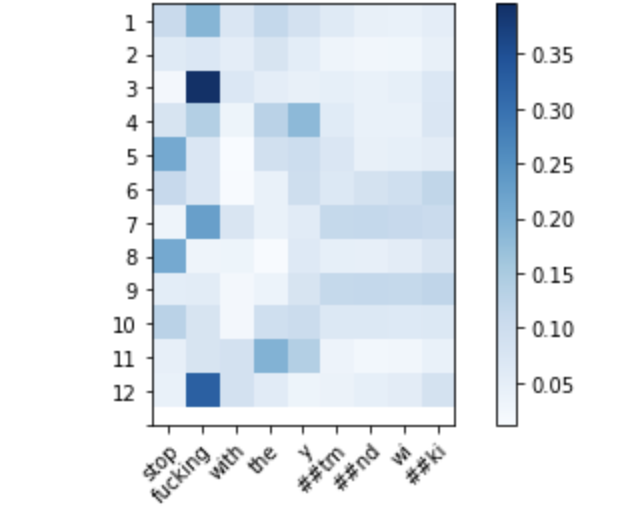
\includegraphics[width=0.60\linewidth]{p1.png} % comment this when submit
	\caption{\bf{Visualization for attention analysis of a toxic sentence} }
	\label{fig1} % label should be on the back of caption, otherwise it shows the error.
\end{figure}

Based on the attention analysis visualization, as we can observe that X-axis is the word tokens/key which attention is being paid, and Y-axis is number of head. The intensity of color blue shows attention weights. As we can observe, the bad words in this sentence have more attention weights higher than 0.35, which can be a good indicator to predict the comment as toxic. General speaking, our model forms a strong composite representations to understand language.

We also tested the BERT model performance with the Kaggle test data which contains 153164 comments. Our model reports a lower Macro F1 score at 0.788, lower than the nice >0.90 scores we had on the test split of our training data. We have submitted the predictions to the Kaggle competition which scores differently. It takes in probabilities(sigmoid values) and not the actual 0 and 1 classification labels for the six columns. The evaluation metric is mean column-wise ROC AUC, according to the competition page. The graded score is 0.97905 and such a score ranked about 2586 on the public leaderboard among 4500+ entries.


\section{Conclusion}

In a word, the best combination of our model is batch size of 32, epochs of 2 and learning rate of 2e-5 which we will obtain F1-score of 0.905.
Beisdes, BERT model performs aproximately 4\% better than the baseline LSTM model.


We also encounter some challenges. One of the challenges we face is that this is not a binary or a simple multi-class classification problem where every comment can only be attributed to one class. A comment can be attributed to more than one class which meant we cannot use softmax in a typical way. The immediate solution was to have 6 different models where every model will be a binary classifier for one class predicting if the comment can or cannot be attributed to that specific class. However, this was very inefficient from a computation standpoint since we would have to use 6 times the memory and storage compared to a single model and also spend way more time iterating on each of the models. The more non-trivial solution we came up with is to use a single newtork for all classifying all the labels and use the BCELoss along with the Sigmoid activation function to predict and calculate the loss in one go.

In the future, we will study more on dealing with data imbalance
and also we would like to extend our model to apply XLNet pre-trained model
as well.



%\bibliographystyle{splncs04}
\bibliographystyle{apalike}
\bibliography{final_project_report}
\end{document}
